%TODO dopisać coś więcej dlaczego mniejsze komórki nie są potrzebne.
% skala  budynku to że nie interesuje nas jak dokładnie będzie się palić każde 10cm^3 ale 
% jak ogień będzie się przemieszczał. rozmiar człowieka z perełek
%TODO w sekcji gdzie będziemy się chwalić wynikami algorytmu napisać o zasadzie zachowania energii
%TODO gęstość materiału może się przydać w algorytmie do obliczania masy powietrza po podgrzaniu spr to
\chapter{Algorytm}
\label{cha:Algorytm}
Rozdział przedstawia propozycję algorytmu symulacji rozprzestrzeniania się ognia i dymu podczas pożaru.
Przedstawiony poniżej model jest niehomogenicznym automatem komórkowym i jako taki spełnia postulat niehomogeniczności.
W pierwszej części rozdziału przedstawiono wartości parametrów tworzących automat komórkowy. Kolejne podrozdziały 
zawierają szczegółowy opis kluczowych funkcji współtworzących funkcję przejścia.
% Plan rozdziału
% 1. Jaki typ automatu 3D. wielkość - określana przez usera
% 2. Kształt komórek i wielkość komórek
% 3. Sąsiedztwo - nieregularne, inni sąsiedzi przy krawędziach
% 4. Zbiór stanów
% 5. Funkcja przejścia
% 6. W kolejnych podrozdziałach funkcje będące czynnikami funkcji przejścia - przewodnictwo, konwekcja, dym
% 7. Rodzaje komórek. problem wąskich drzwi i jego rozwiązanie
\section {Model automatu}
Zgodnie ze wzorem \ref{def_automatu} będącym istotą przytoczonej w rozdziale \ref{cha:Automaty komórkowe} definicji automatu komórkowego według Weimara jednym z kluczowych elementów podczas tworzenia automatu jest określenie siatki, czyli powierzchni automatu. W modelu symulacji pożaru w budynku
ze względu na trójwymiarowość zjawiska oraz istotę jego rzeczywistego odtworzenia (możliwość wykorzystania wyników w celu
opracowania modelu ewakuacji osób, badanie przyczyn katastrofy i drogi rozchodzenia ognia) najbardziej naturalnym typem automatu 
jest automat \textsl {trójwymiarowy}. Powierzchnię automatu stanowi sześcian składający się z również sześciennych komórek o wymiarach $0.5m x 0.5m x 0.5m$.Odpowiedni dobór wielkości komórek automatu ma kluczowy wpływ na jego działanie. Zbyt mała ilość komórek może doprowadzić do utraty
dokładności algorytmu oraz ukazać zniekształcony obraz działania modelu. Zbyt duża ilość elementów powoduje spadek wydajności algorytmu, a w komputerowej realizacji algorytmu oznacza zwiększone zapotrzebowanie na pamięć i moc procesora. W omawianym algorytmie
wielkość komórek została wybrana empirycznie.
Wybrany na podstawie doświadczeń rozmiar komórki jest najlepszym
kompromisem między czasem działania a dokładnością modelu.
Rozmiar całkowitej powierzchni automatu jest wielkością zmienną, definiowaną przez użytkownika systemu. Pozwala to na przeprowadzanie symulacji budynków o zróżnicowanej wielkości dopasowując rozmiar automatu tak aby całość
siatki stanowiła budynek oraz aby budynek był w całości objęty przez siatkę. 



Typy komórek wchodzących w skład automatu można podzielić na dwie zasadnicze grupy:
\begin{itemize}
\item Ciała stałe
\item Gazy
\end{itemize}
Model symulacji nie uwzględnia interakcji ognia z wodą lub innymi cieczami i nie przedstawia zjawisk fizycznych zachodzących podczas tych interakcji.
W ciałach stałych funkcje przejścia odzwierciedlają zjawisko przewodnictwa cieplnego. W gazach będących płynami przewodnictwo zastąpione jest konwekcją.
Wszystkie typy komórek poddane są zjawisku radiacji.
Ponadto, komórki reprezentujące ciała stałe dzielimy ze względu na rodzaj materiału z jakiego są stworzone.


Każdy z materiałów posiada zestaw parametrów określających jego właściwości fizyczne:
\begin{itemize}
\item Ciepło właściwe - określa jak zmienia się temperatura ciała w zależności od ilości dostarczonego / oddanego ciepła
\item Gęstość
\item Współczynnik przewodnictwa ciepła - określa zdolność materiału do przewodnictwa cieplnego
\item Temperatura zapłonu - określa temperaturę charakterystyczną dla danego materiału, po której osiągnięciu 
	dochodzi do produkcji palnych oparów
\item Palność - określa procentową ilość oparów powstałych po osiągnięciu temperatury zapłonu. Determinuje szybkość spalania.
\end{itemize}
Wyżej wymienione parametry bezpośrednio wpływają na zachowanie funkcji przejścia, powodując zróżnicowane zachowanie komórek w zależności od typu materiału.


Poza różnymi typami komórek, o niehomogeniczności automatu świadczą różne definicje sąsiedztwa.
Ze względu na fakt, że siatka automatu modeluje przestrzeń zamkniętą - budynek - konieczne jest zróżnicowanie sąsiedztwa w środku siatki oraz na jej brzegach.
W zaproponowanym algorytmie wykorzystano zmienną liczbę sąsiadów w zależności od położenia komórki. 
Komórka znajdująca się w środku siatki posiada sześciu sąsiadów. Sąsiadami są komórki przylegające ścianami do aktualnie
rozpatrywanej, co jest trójwymiarowym wariantem sąsiedztwa von Neumana. %TODO Jacek dopisać coś z Wolframa czemu mniej sąsiadów wystarcza, a więcej
% wcale nie poprawia sytuacji a jest zbędnymi obliczeniami
 Rozkład sąsiadów dla komórki znajdującej się w centrum przestrzeni przedstawia rysunek \ref{sasiedzi}.
\begin{figure}
\begin {center}
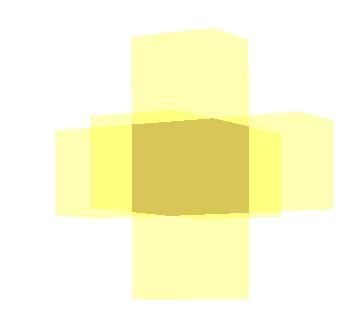
\includegraphics{sasiedztwo.jpg} \\
\caption { Schemat sąsiedztwa}
\label {sasiedzi}
\end {center}
\end{figure}
W przypadku gdy komórka znajduje się na skraju siatki liczba sąsiadów ulega zmniejszeniu. Do zbioru sąsiadów należą komórki, przylegające ścianami do 
rozpatrywanej oraz jednocześnie będące wewnątrz przestrzeni modelu. W skrajnym przypadku, gdy komórka znajduje się w narożniku liczba sąsiadów z sześciu spada
do trzech. Stan komórki brzegowej jest obliczany, podobnie jak w przypadku komórki znajdującej się wewnątrz automatu na podstawie wszystkich jej sąsiadów. Zmniejszona ilość sąsiadów powoduje zmieniony rozkład ich wpływu na nowy stan bieżącej komórki. Waga znaczenia każdej z komórek wzrasta dwukrotnie.
Innymi, alternatywnymi rozwiązaniami sytuacji brzegowych są :
\begin {enumerate}
\item Uznanie za sąsiada ostatniego elementu w danej płaszczyźnie, elementu pierwszego czyli znajdującego się na przeciwległym brzegu. Jest to tak zwane sąsiedztwo
periodyczne. W przypadku symulacji pożaru taki tym sąsiedztwa nie odzwierciedla rzeczywistych interakcji między komórkami w pomieszczeniu. Komórka znajdująca się 
po drugiej stronie budynku nie wpływa bezpośrednio na stan aktualnie rozpatrywanej.
\item Zastosowanie warunków pochłaniających, czyli nadanie komórkom brzegowym z góry określonego, nie uwzględniającego sąsiedztwa stanu. Rozwiązanie to 
powoduje, że komórki brzegowe nie mogą być traktowane jako elementy budynku z rzeczywistymi właściwościami fizycznymi.
\end{enumerate}

Każda z komórek automatu może przyjmować jeden z trzech stanów:
\begin{itemize}
\item Komórka niezapalona
\item Komórka paląca się
\item Dym
\end{itemize}
Poza wyżej wymienionymi trzema stanami, każda komórka posiada wartość swojej aktualnej temperatury, która również w sposób pośredni określa jej stan i ma znaczący
wpływ na wynik funkcji przejścia.

